\appendix
\section{High order accurate base scheme}\label{sec:ho}
This section provides a framework to extend the method of lines finite volume scheme to high order.  
%The high order state redistribution could also be applied to a high order MUSCL scheme but we do not do this here.  
In Section \ref{sec:ho_basescheme}, we describe the high order method of lines scheme.  This base scheme requires a high order polynomial reconstruction on each cell of the base grid described in Sections \ref{sec:ho_reconstruction} and \ref{sec:ho_reconstruction_primitive}.


\subsection{Method of lines} \label{sec:ho_basescheme}


High order accuracy in space is achieved by reconstructing a high order polynomial on each cell and using it to evaluate the numerical flux at the face quadrature points (Figure \ref{fig:2dfig}).  
For third and fourth order accurate schemes, we use the two-point Gauss
Legendre quadrature rule illustrated by squares in Figure \ref{fig:2dfig_ho_vquad}.  Our
numerical experiments again use the local Lax-Friedrichs flux function.

The high order method of lines scheme requires quadrature rules on volumes for 
\begin{enumerate}
	\item the computation of cell averages for the initial condition $\mathbf{U}^0$,
	\item geometrical constants used in polynomial reconstruction (Sections \ref{sec:ho_reconstruction} and \ref{sec:ho_reconstruction_q}),
	\item reconstruction in primitive variables (Section \ref{sec:ho_reconstruction_primitive}).
\end{enumerate}

On cut cells, integrals are computed by first triangulating the cut cell, then using a quadrature rule of sufficient order on each subtriangle.  The triangulation is not necessarily Delaunay and we do not introduce new vertices to triangulate the cut cells.  This approach can result in thin and small triangles on the cut cell (Figure \ref{fig:2dfig_ho_vquad}).  It is simple to show that the accuracy of volume integrals approximated in this manner on cut cells will not be affected \cite{QIN201324}.
On full cells, we use quadrature rules designed for quadrilaterals.  

\begin{figure}
	\begin{center}
		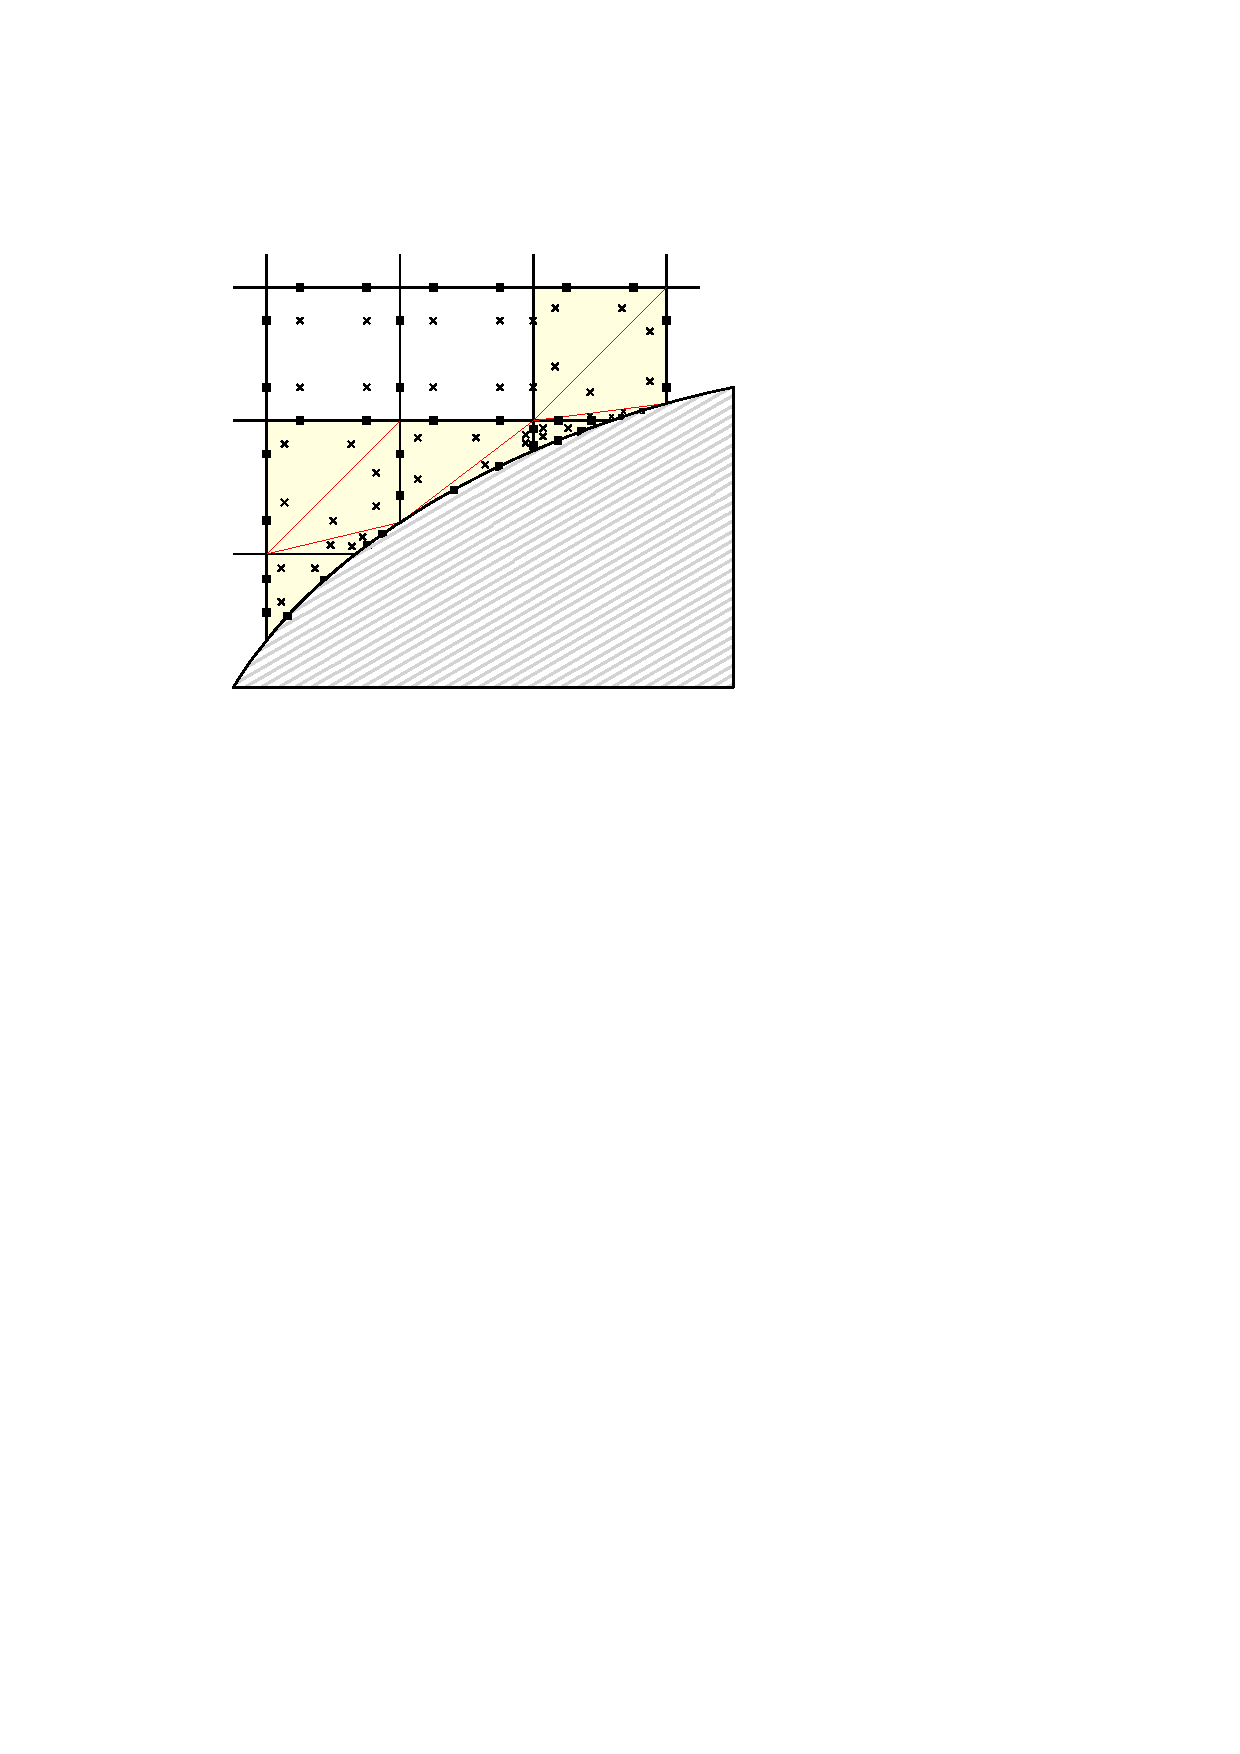
\includegraphics[width=3.0in]{figs/example_ccmesh_ho_vquad.pdf}
		\caption{\sf 
%			The high order method of lines scheme reconstructs to Gauss-Legendre quadrature points. 
			The two-point Gauss-Legendre quadrature points used for third and fourth order methods are indicated by a square ($\blacksquare$).  The triangulations used for volume integration on cut cells are indicated by red lines and the volume quadrature points for third and fourth order methods are indicated by a cross ($\times$).} 
		\label{fig:2dfig_ho_vquad}
	\end{center}
\end{figure}


High order accuracy in time is obtained by applying a Runge-Kutta method   
with the same degree accuracy in time  as the spatial reconstruction.
%We use the two stage TVD-RK2 scheme in \eqref{eq:molscheme} with linear reconstructions and the time step restriction given in \eqref{eq:vn1}.
For the third order method, we use the three stage TVD-RK3 method
%\begin{equation}\label{eq:molscheme_ho2}
%\begin{aligned}
%\mathbf{U}^{(1)} &= \mathbf{U}^{n} + \Delta t L(\mathbf{U}^n), \\
%\mathbf{U}^{(2)} &=  \frac{3}{4}\mathbf{U}^{n} + \frac{1}{4}(\mathbf{U}^{(1)} + \Delta t L(\mathbf{U}^{(1)})), \\
%\mathbf{U}^{(3)} &= \mathbf{U}^{(2)} + \Delta t L(\mathbf{U}^{(2)}),  \\
%\mathbf{U}^{n+1} &= \frac{1}{3}\mathbf{U}^{n} + \frac{2}{3}\mathbf{U}^{(3)}  ,	
%\end{aligned}
%\end{equation}
with the time step restriction
\begin{equation}
\Delta t \left( \frac{|a|}{\Delta x} + \frac{|b|}{\Delta y} \right) \leq 1.6,
\end{equation}
where $(a,b)$ are the wave speeds.
Note that this L2 stability limit is larger the SSP limit.
For the fourth order method, we use the standard four stage Runge-Kutta
scheme.
%since a four-stage TVD\_RK4 scheme does not exist..
%\begin{equation}\label{eq:molscheme_ho4}
%\begin{aligned}
%\mathbf{k}^{(1)} &= \Delta t L(\mathbf{U}^n), \\
%\mathbf{k}^{(2)} &= \Delta t L \left(\mathbf{U}^n + \frac{\Delta t}{2} \mathbf{k}^{(1)} \right), \\	
%\mathbf{k}^{(3)} &= \Delta t L \left(\mathbf{U}^n + \frac{\Delta t}{2} \mathbf{k}^{(2)} \right), \\	
%\mathbf{k}^{(4)} &= \Delta t L \left(\mathbf{U}^n + \Delta t \mathbf{k}^{(3)} \right), \\	
%\mathbf{U}^{n+1} &=\mathbf{U}^n + \frac{1}{6}(\mathbf{k}^{(1)} + \mathbf{k}^{(2)}+ \mathbf{k}^{(3)}+ \mathbf{k}^{(4)}),
%\end{aligned}
%\end{equation}
%and the time step restriction
%\begin{equation}
%\Delta t \left( \frac{|a|}{\Delta x} + \frac{|b|}{\Delta y} \right) \leq 1.2.
%%\end{equation}
%For both third and fourth order accurate methods, we have obtained their associated time step restrictions by numerical evaluation of the amplification factor resulting from a linear stability analysis.
%since a four-stage TVD-RK4 scheme does not exist
%\begin{figure}
%	\begin{center}
%		\includegraphics[width=3.0in]{figs/example_ccmesh_ho.pdf}
%		\caption{\sf Example base grid in two space dimensions. The cells shaded in yellow are the cut cells. The high order method of lines scheme reconstructs to Gauss-Legendre quadrature points.  We have indicated by the hollow cross ($\square$) the two-point Gauss-Legendre quadrature points used for reconstructions of degree $d=2,3$.} 
%		\label{fig:2dfig_ho}
%	\end{center}
%\end{figure}
%For these schemes, we use the following time step restriction
%\begin{equation}
%\Delta t   \max_{i,j}\left( \frac{|a_{i,j}|}{\Delta x} + \frac{|b_{i,j}|}{\Delta y} \right) \leq 1.
%\end{equation}


%It has been proven that this approach does not affect the accuracy

%In what follows, volume integrals are computed with quadrature rules of order $p$, when the scheme accuracy is of order $p$.

For higher order methods, the boundary conditions also have to be higher
order or the solution deteriorates. For order 3 and higher we use
the curved boundary conditions in Algorithm 2 from \cite{KB:2006}.


\subsection{Polynomial reconstruction} \label{sec:ho_reconstruction}
On both full and cut cells, the base finite volume scheme requires a reconstructed polynomial of the form
\begin{equation}\label{eq:uu}
\begin{aligned}
u^n_{i,j} (x,y) = U^n_{i,j} +  \sum_{1 \leq |\alpha| \leq d}  \frac{1}{\alpha!} \sigma^n_{\alpha,i,j} [(x- x_{i,j})^{\alpha_1}(y-y_{i,j})^{\alpha_2}- S_{\alpha,i,j}]
\end{aligned}
\end{equation}
where $d$ is the degree of polynomial reconstruction,
$\alpha = (\alpha_1, \alpha_2)$, $|\alpha| = \alpha_1 + \alpha_2$, $\sigma^n_{\alpha,i,j}$ is the $\alpha$th reconstruction coefficient, and $ (x_{i,j}, y_{i,j})$ is the physical centroid of cell $(i,j)$. 
The $  S_{\alpha, i,j}$ are geometric constants given by
$$
S_{\alpha, i,j} = \frac{1}{ V_{i,j}}  \int_{\Omega_{i,j}} 
(x-x_{i,j})^{\alpha_1} \, (y-y_{i,j})^{\alpha_2} ~ dx \, dy .
$$
They enforce that 
\begin{equation} \label{eq:uaverage}
\frac{1}{ V_{i,j}}  \int_{\Omega_{i,j}} u^n_{i,j}(x,y) ~dx\,dy = U^n_{i,j},
\end{equation}
where  $U^n_{i,j}$ is the cell average on cell $i,j$.  On whole cells, 
these constants are
\begin{equation}
	\begin{aligned}
		S_{(1,0)} &= 0, ~ S_{(0,1)} = 0 \\
		S_{(2,0)} &= \frac{1}{12}, ~ S_{(1,1)} = 0, ~ S_{(0,2)} = \frac{1}{12}\\
		S_{(3,0)} &= 0, ~ S_{(2,1)} = 0, ~ S_{(1,2)} = 0, ~ S_{(3,0)} = 0.
	\end{aligned}
\end{equation}
On cut cells, the above constants are precomputed during a mesh preprocessing operation.

On whole cells without cut cells in their reconstruction stencil, the derivatives of $u^n_{i,j}(x,y)$ are computed using standard finite difference formulas of sufficient accuracy.
On cut cells and edge neighbors of cut cells, the derivatives are determined by solving in the least squares sense
\begin{equation}\label{eq:ls_base}
\frac{1}{V_{r,s}}\int_{\Omega_{r,s}} u^n_{i,j}(\mathbf{x})~d\mathbf{x} = U^n_{r,s} \quad \forall (r,s) \in R_{i,j},
\end{equation}
where the reconstruction neighborhoods $R_{i,j}$ depend on the order of approximation of the scheme (Table \ref{tab:reconneigh}).
\begin{table}
	\centering
        \ra{1.2}
	\begin{tabular}{|c|c|}
		\hline 
		Order of accuracy & $R_{i,j}$ and $\hat R_{i,j}$ \\
		\hline
		2 (1st order gradients) &  $3 \times 3 $ \\
		\hline
		2 (2nd order gradients) &  $5 \times 5 $ \\
		\hline
		3 & $5 \times 5$ \\
		\hline
		4 & $7 \times 7$ \\
		\hline
	\end{tabular} 
	\caption{Reconstruction neighborhoods centered on cell $i,j$ used for the base finite volume scheme $R_{i,j}$ and on neighborhoods $\widehat{R}_{i,j}$ in terms of the 
        order of accuracy of the method.   
%	If $i,j$ is cut, then not all cells in, e.g., the $7 \times 7$ neighborhood centered on $i,j$ will exist and thus cannot be included in the least squares system \eqref{eq:ls_base}.
} \label{tab:reconneigh}
\end{table}

The issue of obtaining a well-conditioned derivatives can occur as they do for the second order algorithm (Section \ref{sec:srd_postprocessing}).  Here, we adopt the same proposed remedy, i.e., if the weighted centroids are not at minimum distance apart in the $x$ or $y$ direction then we increase the stencil size for the least squares computation.  These minimum distances are provided in Table \ref{tab:mindist}.  For the third order accurate method, if the $ R_{i,j}$ does not have a cell that is at least $\frac{5}{2}\Delta x$ away from the centroid, we use a $9 \times 7$ neighborhood.
\begin{table}
	\centering
        \ra{1.2}
	\begin{tabular}{|c|c|}
		\hline 
		Order of accuracy & Minimum distance in $x$, $y$ direction
                    \\[.08in] \hline 
		2 (1st order gradients)  & $\frac{1}{2}\Delta x$,
                    $\frac{1}{2}\Delta y$ \\[.08in] \hline 
		2 (2nd order gradients)  & $\frac{3}{2}\Delta x$, 
                     $\frac{3}{2}\Delta y$ \\ [.08in] \hline 
		3 & $\frac{3}{2}\Delta x$, $\frac{3}{2}\Delta y$ \\
                   [.08in] \hline
		4 & $\frac{5}{2}\Delta x$, $\frac{5}{2}\Delta y$ \\ [.08in] \hline 
	\end{tabular}  
	\caption{We require that there be cells in the reconstruction stencils, $R_{i,j}$ and $\widehat R_{i,j}$, that lie at least the above distances from the cell centroid.} \label{tab:mindist}
\end{table}

\subsection{High order reconstruction in primitive variables} \label{sec:ho_reconstruction_primitive}
In this section, we describe how we evaluate the interface states for the numerical fluxes in \eqref{eq:fvscheme} when solving the Euler equations of gas dynamics.  It is well known that gas flow can be difficult to compute when reconstructing and limiting the numerical solution in conserved variables, i.e., $(\rho, \rho u, \rho v, E)$.  Thus, we adopt the common approach of reconstructing the numerical solution in primitive variables $(\rho, u, v, p)$.  First, we reconstruct in conserved variables, i.e., on each cell we obtain a polynomial 
%of degree $p$ 
for $\rho(\mathbf{x})$, $\rho u(\mathbf{x})$, $\rho v(\mathbf{x})$, and $E(\mathbf{x})$.  Next, we compute approximations to the primitive solution averages on each cell, i.e.,
\begin{align} 
\begin{aligned}
u_{i,j} &= \frac{1}{V_{i,j}} \int_{\Omega_{i,j}} \frac{\rho u(\mathbf{x})}{\rho(\mathbf{x})} d\mathbf{x} \\
v_{i,j} &= \frac{1}{V_{i,j}} \int_{\Omega_{i,j}} \frac{\rho v(\mathbf{x})}{\rho(\mathbf{x})} d\mathbf{x} \\
p_{i,j} &= \frac{1}{V_{i,j}}\int_{\Omega_{i,j}} (\gamma-1) \left[E(\mathbf{x}) - \frac{1}{2}\frac{\rho u(\mathbf{x})^2+\rho v(\mathbf{x})^2}{\rho(\mathbf{x})} \right] ~d\mathbf{x}
\end{aligned}\label{eq:primitive}
\end{align}
The above integrals are approximated with quadrature rules that integrate polynomials
of degree $d$ exactly for spatial reconstructions of degree $d$.
Finally, the solution is reconstructed to the cell interfaces in 
primitive variables using the solution averages 
computed in \eqref{eq:primitive}.  

\section{High order state redistribution method} \label{sec:ho_reconstruction_q}


We determine merging neighborhoods, weighted centroids and volumes as in the second order case (Section \ref{sec:preprocessing}).  The few additional details are outlined below.

\subsection{State redistribution postprocessing} \label{sec:postprocessing_ho}
Step 1 of the higher order state redistribution is the same as in the 
second order method described in Section \ref{sec:srd_postprocessing}.  
The method differs in that we reconstruct a high order polynomial 
on each neighborhood as we describe below.


%\subsubsection*{Compute the provisionally updated numerical solution}
%Compute forward Euler update (for the third order method) or intermediate solution value (for the fourth order method) of the method of lines scheme presented in Section \ref{sec:ho_basescheme}, i.e., the update is of the form
%\begin{equation} \label{eq:stage_ho2}
%\widehat{U} = U^n + \Delta t  L(U^n),
%\end{equation}
%where $L$ is the operator that results from the right-hand-side of \eqref{eq:fvscheme} and $\widehat{U}$ is a vector of provisionally updated, unstable solution averages on the entire grid before state redistribution.
%
%
%%The update in \eqref{eq:stage_step} corresponds to one stage of the high order method of.
%
%
%\subsubsection*{Compute weighted solution averages on each neighborhood}
%
%This step is the same as the second order case, i.e., we form the merged solution averages
%\begin{equation}\label{eq:q_avg1}
%\widehat{Q}_{i,j} =  \frac{1}{ \widehat{V}_{i,j}} \,  \sum_{(r,s) \in M_{i,j} }\frac{V_{r,s}}{N_{r,s}} \widehat{U}_{r,s},
%\end{equation}
%\noindent where $M_{i,j}$ is again the set of indices of cells in the 
%merging neighborhood, and the weighted volume of the merged tile 
%\begin{equation}\label{eq:modV}
%\widehat{V}_{i,j} = \sum_{(r,s) \in M_{i,j} }\frac{V_{r,s}}{N_{r,s}} .
%\end{equation}
%The merging neighborhoods are constructed in the same fashion as the second order method.  That
%is, we merge in the normal direction from the boundary until the volume constraint \eqref{eqn:voldef} is satisfied.  If there are not enough cells in the normal direction, we use a centered tile of sufficient area, e.g., $3 \times 3$ tile, or $5 \times 5$ tiles.



\subsubsection*{Step 2. Reconstruct a high order polynomial on each neighborhood}
For high order accuracy in space, we reconstruct a polynomial of degree $p$ on each neighborhood using a least squares procedure.  Similar to the base grid reconstruction is \eqref{eq:uu}, the high order reconstruction on neighborhood $(i,j)$ is of the form
\begin{equation}\label{eq:q}
\begin{aligned}
    \widehat q_{i,j} (x,y) = \widehat{Q}_{i,j} +  \sum_{1 \leq
    |\alpha| \leq d}  \frac{1}{\alpha!} \widehat \sigma_{\alpha,i,j}
    [(x-\widehat x_{i,j})^{\alpha_1}(y-\widehat
    y_{i,j})^{\alpha_2}-\widehat S_{\alpha,i,j}]
\end{aligned}
\end{equation}
where $\alpha = (\alpha_1, \alpha_2)$, $|\alpha| = \alpha_1 + \alpha_2$, $\sigma_{\alpha,i,j}$ is the $\alpha$th reconstruction coefficient,
and $\widehat x_{i,j}$, $\widehat y_{i,j}$ is again the weighted centroid of the merging neighborhood for cell $(i,j)$. 
The $ \widehat S_{\alpha, i,j}$ are  geometric constants given by
$$
\widehat S_{\alpha, i,j} = \frac{1}{ \widehat{V}_{i,j}} \sum_{(r,s) \in M_{i,j} }\frac{V_{r,s}}{N_{r,s}} \int_{\Omega_{r,s}} 
(x-\widehat{x}_{i,j})^\alpha_1 (y-\widehat{y}_{i,j})^\alpha_2 
~d\mathbf{x},
$$
As in \eqref{eq:uu}, the $\widehat S_{\alpha, i,j}$ constants 
ensure that the weighted average of the polynomial 
reconstruction $\widehat q_{i,j}(x,y)$ on the merging neighborhood 
associated to cell $i,j$ is $\widehat{Q}_{i,j}$,
\begin{equation} \label{eq:average}
\frac{1}{ \widehat{V}_{i,j}} \sum_{(r,s) \in M_{i,j} }\frac{1}{N_{r,s}} \int_{\Omega_{r,s}} \widehat{q}_{i,j}(\mathbf{x}) ~d\mathbf{x} = \widehat{Q}_{i,j}.
\end{equation}


The reconstruction coefficients $\widehat \sigma_{\alpha,i,j}$ are computed by solving
\begin{equation}\label{eq:qi}
\frac{1}{\widehat{V}_{r,s}}\sum_{(r',s') \in M_{r,s}}\frac{1}{N_{r',s'}}\int_{\Omega_{r',s'}} \widehat q_{i,j}(\mathbf{x})~d\mathbf{x} = \widehat Q_{r,s} \quad \forall (r,s) \in \widehat R_{i,j},
\end{equation}
in the least squares sense, where $\widehat R_{i,j}$ is the set of
indices of neighborhoods used for reconstruction on merging
neighborhood $(i,j)$, shown in  Table \ref{tab:reconneigh}.  
Unlike the case for linear reconstructions, \eqref{eq:qi} does not
simplify to \eqref{eqn:linrecon} where we could use only the  
weighted centroids; we have to evaluate the integral instead.
Note that there are 5 and 9 reconstruction coefficients $\widehat{\sigma}_{\alpha, i,j}$, when the order of accuracy is three and four, respectively.

\subsubsection*{Step 3. Final solution update}
The final solution update on cell $(i,j)$ is
	\begin{equation}\label{eq:final_update}
	U^{n+1}_{i,j} =  \frac{1}{V_{i,j}}\sum_{(r,s) \in W_{i,j}}\frac{1}{N_{i,j}}\int_{\Omega_{i,j}} \widehat q_{r,s}(\mathbf{x})~d\mathbf{x} ,
	\end{equation}
	where $W_{i,j}$ is a set of merging neighborhoods to which cell $(i,j)$ belongs.
%\end{enumerate}
The integrals in \eqref{eq:qi} and \eqref{eq:final_update} are computed exactly on both full and cut cells.  

\textit{Note}: for the third order accurate method, $U^{n+1}_{i,j}$ corresponds to a stage of the TVD-RK3 scheme.  
When stabilized by state redistribution, the method of lines scheme becomes
\begin{equation}\label{eq:molscheme_ho2_srd}
\begin{aligned}
\mathbf{U}^{(1)} &= S\left(\mathbf{U}^{n} + \Delta t L(\mathbf{U}^n) \right), \\
\mathbf{U}^{(2)} &=  \left(\frac{3}{4}\mathbf{U}^{n} + \frac{1}{4}S(\mathbf{U}^{(1)} + \Delta t L(\mathbf{U}^{(1)})) \right), \\
\mathbf{U}^{(3)} &= S\left(\mathbf{U}^{(2)} + \Delta t L(\mathbf{U}^{(2)}) \right),  \\
\mathbf{U}^{n+1} &= \frac{1}{3}\mathbf{U}^{n} + \frac{2}{3}\mathbf{U}^{(3)},	
\end{aligned}
\end{equation}
where $S$ is the linear state redistribution operator applied after each forward Euler step of the TVD-RK3 scheme.
For the fourth order accurate method, $U^{n+1}_{i,j}$ corresponds to an intermediate 
solution value of a four stage RK4 scheme.  Thus, when stabilized by state redistribution, 
it becomes 
\begin{equation}\label{eq:molscheme_ho4_srd}
\begin{aligned}
\mathbf{k}^{(1)} &= \Delta t L(\mathbf{U}^n), \\
\mathbf{k}^{(2)} &= \Delta t L \left(S\left(\mathbf{U}^n + \frac{\Delta t}{2} \mathbf{k}^{(1)}\right) \right), \\	
\mathbf{k}^{(3)} &= \Delta t L \left(S\left(\mathbf{U}^n + \frac{\Delta t}{2} \mathbf{k}^{(2)}\right) \right), \\	
\mathbf{k}^{(4)} &= \Delta t L \left(S\left(\mathbf{U}^n + \Delta t \mathbf{k}^{(3)} \right) \right), \\	
\mathbf{U}^{n+1} &= S\left(\mathbf{U}^n + \frac{1}{6}(\mathbf{k}^{(1)} + \mathbf{k}^{(2)}+ \mathbf{k}^{(3)}+ \mathbf{k}^{(4)})\right).
\end{aligned}
\end{equation}


%\subsection{Conservation}\label{sec:cons}
%\begin{figure}
%	\centering
%	\includegraphics[width=0.5\textwidth]{figs/simple_example.pdf}
%	\caption{Simple nonuniform grid of three cells where $\Omega_2$ is the small cell and $\Omega_1$ and $\Omega_3$ are large cells.  The red arrows indicate the merging neighborhoods associated to each cell in the grid.}\label{fig:simple_example}
%\end{figure}
%The total mass of the numerical solution at $t^{n+1}$ is
%\begin{equation}\label{eq:total_mass}
%\mathcal{M}^{n+1} = \sum_{i,j} V_{i,j} U^{n+1}_{i,j}.
%\end{equation}
%From the general form of the state redistribution algorithm 
%in \eqref{eq:final_update}, the total mass in \eqref{eq:total_mass} can also be written as a sum of mass contributions from each merging neighborhood, i.e.,
%\begin{equation}\label{eq:total_mass2}
%\mathcal{M}^{n+1} = \sum_{i,j} \widehat{\mathcal{M}}_{i,j},
%\end{equation}
%where the mass contribution of merging neighborhood $(i,j)$ is
%\begin{equation}\label{eq:mi}
%\widehat{\mathcal{M}}_{i,j} = \sum_{k \in M_{i,j}}\frac{1}{N_{k}} \int_{\Omega_{k}}\widehat q_{i,j}(\mathbf{x}) ~d\mathbf{x},
%\end{equation}
%and $\widehat q_{i,j}(x)$ is that neighborhood's polynomial reconstruction.  
%To illustrate this, consider the simple one dimensional grid in figure \ref{fig:simple_example} composed of three cells, $\Omega_1$, $\Omega_2$, and $\Omega_3$, where $\Omega_2$ is the only small cell.  The red arrows indicate the associated merging neighborhoods, i.e., the merging neighborhood of $\Omega_2$ comprises all three cells.
%Substituting the final solution update \eqref{eq:final_update} into \eqref{eq:total_mass}, the total mass of the numerical solution on this grid can be written
%\begin{equation}
%	\mathcal{M}^{n+1} = \frac{1}{2}\left( \int_{\Omega_1} \widehat q_1(x)~dx +  \int_{\Omega_1} \widehat q_2(x)~dx \right) + \int_{\Omega_2} \widehat q_2(x)~dx + \frac{1}{2} \left( \int_{\Omega_3} \widehat q_2(x)~dx +  \int_{\Omega_3} \widehat q_3(x)~dx \right)
%\end{equation}
%Regrouping terms, the total mass can be rewritten in terms of mass contributions from each merging tile, i.e.,
%\begin{equation}
%\mathcal{M}^{n+1} = \underbrace{\frac{1}{2} \int_{\Omega_1} \widehat q_1(x)~dx}_{\widehat{\mathcal{M}}_{1}} + \underbrace{\frac{1}{2} \int_{\Omega_1} \widehat q_2(x)~dx  + \int_{\Omega_2} \widehat q_2(x)~dx + \frac{1}{2}  \int_{\Omega_3} \widehat q_2(x)~dx}_{\widehat{\mathcal{M}}_{2}} +  \underbrace{\int_{\Omega_3} \widehat q_3(x)~dx}_{\widehat{\mathcal{M}}_{3}}.
%\end{equation}
%Thus, the respective mass contribution of merging neighborhoods 1, 2, and 3, are
%\begin{align*}
%	\widehat{\mathcal{M}}_{1} & = \frac{1}{2} \int_{\Omega_1} \widehat q_1(x)~dx, \\
%	\widehat{\mathcal{M}}_{2} & =  \frac{1}{2}\int_{\Omega_1} \widehat q_2(x)~dx +  \int_{\Omega_2} \widehat q_2(x)~dx +\frac{1}{2}\int_{\Omega_3} \widehat q_2(x)~dx, \\
%	\widehat{\mathcal{M}}_{3} & = \frac{1}{2}\int_{\Omega_3} \widehat q_3(x)~dx.
%\end{align*}
%With the above in mind, we now return to proving mass conservation on a general two dimensional cut cell mesh.
%
%From \eqref{eq:average}, the mass contribution from an arbitrary tile in \eqref{eq:mi} can be written
%\begin{equation}\label{eq:mi1}
%\widehat{\mathcal{M}}_{i,j} = \widehat Q_{i,j} \widehat V_{i,j}.
%\end{equation}
%% \subsection{First order algorithm}
%% When $\widehat q_i(x)$ is constant, i.e. $\widehat q_i(x) = \widehat Q_i$ by \eqref{eq:q_avg} and Step 2 in Section \ref{sec:first_order}, \eqref{eq:mi} becomes 
%% Substituting \eqref{eq:mi} into \eqref{eq:total_mass2}, we have
%% \begin{equation}\label{eq:mi1}
%% \widehat{\mathcal{M}}_i = \widehat Q_i \widehat V_i.
%% \end{equation}
%% by \eqref{eq:q_avg} in the first order algorithm, by \eqref{eq:pq2} in the second order algorithm, and by \eqref{eq:q2} in the third order algorithm.
%Using the definition of the merging tile average in \eqref{eq:q_avg1}, \eqref{eq:mi1} becomes
%\begin{equation}\label{eq:mi2}
%\widehat{\mathcal{M}}_{i,j} = \sum_{k \in M_{i,j} }\frac{V_k}{N_{k}} \widehat U_{k}.
%\end{equation}
%Substituting \eqref{eq:mi2} into the expression for the total mass in terms of tile contributions \eqref{eq:total_mass2}, the mass at $t^{n+1}$ is
%\begin{equation}\label{eq:totalsum}
%\mathcal{M}^{n+1} = \sum_{i,j} \sum_{k \in M_{i,j} }\frac{V_k}{N_{k}} \widehat U_{k}.
%\end{equation}
%Since $N_k$ indicates the number of times a cell is overlapped by merging neighborhoods, it follows that the $\frac{V_k}{N_{k}} \widehat U_{k}$ term is repeated $N_k$ times in the sum of \eqref{eq:totalsum}.  Thus, we have that the total mass is
%\begin{equation} \label{eq:final}
%\mathcal{M}^{n+1} = \sum_{i,j} h_{i,j} \widehat U_{i,j},
%\end{equation}
%which demonstrates that $\mathcal{M}^{n+1}  = \mathcal{M}^{n} $.
%
%It may not be immediately obvious how \eqref{eq:totalsum} becomes \eqref{eq:final}, so consider again the simple one dimensional example in figure \ref{fig:simple_example}.  The total mass on this simple grid according to \eqref{eq:totalsum} is
%\begin{equation} \label{eq:massexample}
%\mathcal{M}^{n+1} = \underbrace{ \frac{V_1}{2} \widehat U_1 }_{ \widehat{\mathcal{M}}_1 }  + \underbrace{ \left( \frac{V_1}{2} \widehat U_1 + V_2 \widehat U_2 + \frac{V_3}{2} \widehat U_3 \right) }_{ \widehat{\mathcal{M}}_2 }+ \underbrace{ \frac{V_3}{2} \widehat U_3 }_{\widehat{\mathcal{M}}_3}.
%\end{equation}
%Again, $N_k$ indicates the number of times $\frac{V_k}{N_{k}} \widehat U_{k}$ term is repeated in \eqref{eq:totalsum}.  On cell $\Omega_1$, we have $N_1=2$, thus $\frac{V_1}{2} \widehat U_1$ is repeated twice in \eqref{eq:massexample}.  When added together, these two terms become simply $V_1 \widehat U_1$.  The same argument can be applied to the other terms in the sum.  Thus, after simplifying \eqref{eq:massexample}, the total mass is
%$$
%\mathcal{M}^{n+1} = V_1 \widehat U_1 + V_2 \widehat U_2 + V_3 \widehat U_3,
%$$
%which is in the form of \eqref{eq:final}.

\subsection{High-order supersonic vortex study}

To illustrate the higher order SRD algorithm, we continue the convergence 
study of the supersonic vortex problem in Section \ref{sec:ssv}, 
extending it to use a 3rd order and 4th order MOL and SRD scheme.  Here,
the $L_1$ norm of the error in density on the volume is, 
$$
\sum_{i,j}\int_{\Omega_{i,j}}|\rho(x,y) - \rho_{i,j}(x,y)|~dx~dy,
$$
and
$$
\sum_{i,j}\int_{i,j \in \partial \Omega}|\rho(x,y) - \rho_{i,j}(x,y)|~dl,
$$
is the $L_1$ norm of the boundary error in density.
In both cases the numerical solution is reconstructed to the quadrature points.
and the integral is approximated with a quadrature rule, 
We observe the expected rate of convergence in the $L_1$ norm on the volume and a slower convergence rate in the cut cells.

{\small 
\begin{table}[h]
\centering
\hspace*{-.3in}
\subfloat[$L_1$ volume errors.\label{tab:hoL1vol}]{
\begin{tabular}{|l|c|l|l||l|l|}
\hline
$h$ & $N_x ,N_y$ & \multicolumn{2}{|c||}{3rd order} & \multicolumn{2}{|c|}{4th order} \\
\hline
& & LTS & SRD & LTS & SRD \\
\hline
.5297 & 27 & 2.68e-003  & 2.75e-003   & 1.29e-003 &  1.20e-003 \\
\hline
.2648 & 54  & 3.86e-004 (6.9)  & 3.80e-004 (7.2)  & 8.41e-005 (15.3) & 8.36e-005 (14.3) \\
\hline
.1324 & 108 & 5.18e-005 (7.4)  & 5.00e-005 (7.6)  & 5.65e-006 (14.8) & 5.29e-006 (15.8) \\
\hline
.662E-2 & 216 &  ()  & 6.48e-006 (7.7)  &  () & 3.39e-007 (15.6) \\
\hline
\end{tabular}
} 
\quad
\vspace*{.2in}

\hspace*{-.3in}
\subfloat[$L_1$ boundary errors. \label{tab:hoL1bndry}]{
\begin{tabular}{|l|c|l|l||l|l|}
\hline
$h$ & $N_x ,N_y$ & \multicolumn{2}{|c||}{3rd order} & \multicolumn{2}{|c|}{4th order} \\
\hline
& & LTS & SRD & LTS & SRD \\
\hline
.5297 & 27 &  4.81e-002  & 4.94e-002   &    1.73e-002     &  1.45e-002 \\
\hline
.2648 & 54  & 9.14e-003 (5.2)   & 9.47e-003 (5.2)  & 2.38e-003 (7.2) & 2.26e-003 (6.4) \\
\hline
.1324 & 108 & 2.08e-003 (4.3)  & 2.09e-003 (4.5)  & 2.48e-004 (9.5) & 2.29e-004 (9.8) \\
\hline
.662E-2 & 216 &  ()  & 4.69e-004 (4.4)  & () & 2.65e-005 (8.6) \\
\hline
\end{tabular}
}
\caption{\sf  Supersonic vortex example using 3rd and 4th order accurate
method of lines and state redistribution. As before, the volume error
shows the expected order of convergence, and the boundary error has a
reduced convergence rate.}
\end{table}
}

Also as before, in Tables  \ref{tab:hoL1vol} and \ref{tab:hoL1bndry}  
we compare local time-stepping (LTS)  with SRD,  to see if the
latter has any negative effect on the solution. The results are essentially identical,
showing no clear prefrence for which is slightly more accurate at a given resolution.
We conclude again that SRD maintains the accuracy of the underlying base scheme
